\documentclass{article}
\usepackage[spanish]{babel}
\usepackage[utf8]{inputenc}
\usepackage{graphicx}
\usepackage{minted}
\usepackage{courier}

\title{\textbf{Criptografía aplicada: Función SHA-256}}
\author{Javier Domínguez Gómez \\
\small{jdg@member.fsf.org} \\
\small{Fingerprint: 94AD 19F4 9005 EEB2 3384 C20F 5BDC C668 D664 8E2B}}
\date{v0.1.07 - Marzo 2019}

\begin{document}
\maketitle

\tableofcontents{}

\section{Introducción}
    Este documento describe en detalle las características y el funcionamiento logico-matemático de la función \textit{hash} criptográfica o algoritmo SHA-256.
    
    \vspace{3mm}
    Se trata de una función \textit{hash} iterativa y unidireccional que puede procesar datos de entrada, como un cadena de texto o un archivo, para producir una representación condensada de longitud fija llamada \textit{digest}. Este algoritmo determina de la integridad de los datos de entrada, es decir, cualquier cambio en los datos de entrada producirá un \textit{digest} diferente. Esta propiedad es útil en la generación y verificación de firmas digitales y códigos de autenticación de mensajes, así como la generación de números aleatorios o \textit{bits}.
    
    \vspace{3mm}
    Los puntos que vienen a continuación detallan cada uno de los elementos que forman parte del algoritmo empleado en la función \textit{hash} SHA-256, tales como variables, constantes y funciones, y también el desarrollo y explicación de las operaciones de lógica proposicional, álgebra y operaciones con \textit{bits} que se utilizan para obtener el mensaje \textit{digest} adecuado.

\section{Mensaje $M$ o datos de entrada}
    Es la información que procesará la función SHA-256 para calcular el \textit{digest} o \textit{hash} correspondiente. $M$ puede tener longitud variable\footnote{El esquema de relleno que utiliza SHA-256 requiere que el tamaño de la entrada se exprese como un número de 64 bits, es decir: $(2^{64}-1)/8 \approx 2.091.752$ terabytes.}, puede ser un archivo, una cadena de texto como \textit{"Hola mundo"} e incluso una cadena vacía, obteniendo como resultado una cadena $\omega$ de 256 bits de longitud expresada en 64 caracteres hexadecimales o base 16.
        \begin{figure}[H]
        \centering
            $sha256(M) = |\omega|^{64}_{16}$
        \end{figure}
        
        \begin{figure}[H]
        \centering
            $\begin{array}{rcl}
                 sha256('Hola \ mundo') & = & \left \{
                \begin{array}{c}
                    \texttt{ca8f60b2cc7f05837d98b208b57fb648} \\
                    \texttt{1553fc5f1219d59618fd025002a66f5c}
                \end{array}
                \right .
            \end{array}$
        \end{figure}
        
    La cadena hexadecimal generada se obtiene mediante una serie de cálculos en los que se emplean entre otros datos los bits de entrada, es decir, para un mismo mensaje $M$ siempre se obtendrá el mismo \textit{hash} criptográfico. Por el contrario, si se modifica un solo \textit{bit}, por ejemplo cambiando o añadiendo un carácter (los espacios y los saltos de línea también son caracteres), se obtendrá un \textit{hash} distinto.
        \begin{figure}[H]
        \centering
            $\begin{array}{rcl}
                sha256('Hola \ mundo.') & = & \left \{
                \begin{array}{c}
                    \texttt{8a3b7da2428acbc74623fb5a7b306a83} \\
                    \texttt{b62b513371171e78c048fc12fbdb6ddf}
                \end{array}
                \right . \\
                 & \\
                 sha256('abc') & = & \left \{
                \begin{array}{c}
                    \texttt{ba7816bf8f01cfea414140de5dae2223} \\
                    \texttt{b00361a396177a9cb410ff61f20015ad}
                \end{array}
                \right . \\
                 & \\
                 sha256('Abc') & = & \left \{
                \begin{array}{c}
                    \texttt{06d90109c8cce34ec0c776950465421e} \\
                    \texttt{176f08b831a938b3c6e76cb7bee8790b}
                \end{array}
                \right .
            \end{array}$
        \end{figure}
    De este modo, se garantiza la integridad de los datos. Si estos cambian también lo hará el \textit{hash}.

    \subsection{Conversión a hexadecimal}
        Para procesar el mensaje de entrada $M$ hay que realizar en primer lugar una conversión a formato hexadecimal de la misma. En este proceso se ha de sustituir cada carácter ASCII por su número hexadecimal equivalente. Esta información se puede consultar en una tabla ASCII\footnote{https://www.ieee.li/computer/ascii.htm}. Véase el siguiente ejemplo:
            \begin{figure}[H]
            \centering
                $\begin{array}{lclcl}
                \underline{Char} &  & \underline{Dec} &  & \underline{Hex} \\
                H & \Rightarrow & 72 & \Rightarrow & 48 \\
                o & \Rightarrow & 111 & \Rightarrow & 6f \\
                l & \Rightarrow & 108 & \Rightarrow & 6c \\
                a & \Rightarrow & 97 & \Rightarrow & 61 \\
                  & \Rightarrow & 32 & \Rightarrow & 20 \\
                m & \Rightarrow & 109 & \Rightarrow & 6d \\
                u & \Rightarrow & 117 & \Rightarrow & 75 \\
                n & \Rightarrow & 110 & \Rightarrow & 6e \\
                d & \Rightarrow & 100 & \Rightarrow & 64 \\
                o & \Rightarrow & 111 & \Rightarrow & 6f
                \end{array}$
            \end{figure}
        Uniendo cada código hexadecimal correspondiente a cada carácter se obtiene la conversión del mensaje de entrada a hexadecimal o base 16. Nótese que los espacios en blanco, o los signos de puntuación si los hubiere, también son caracteres ASCII, por lo tanto también tienen una equivalencia numérica.
            \begin{figure}[H]
            \centering
                $\begin{array}{rcl}
                    Hola \ mundo & = & \texttt{486f6c61206d756e646f} \\
                    abc & = & \texttt{616263} \\
                    Te \ gusta \ cifrar? & = & \texttt{5465206775737461206369667261723f} \\
                \end{array}$
            \end{figure}
        Una vez se obtiene el mensaje de entrada en formato hexadecimal se ha de reservar el resultado a parte para utilizarlo más adelante en otras funciones.

    \subsection{Cálculo de la longitud de $M$}
        En el proceso para hallar el \textit{digest} o \textit{hash}, será necesario calcular la longitud del mensaje de entrada $|M|$. Primero hay que calcular la longitud en \textit{bits}. Lo más sencillo es multiplicar el número total de caracteres ASCII del mensaje de entrada por 8, ya que cada carácter ASCII equivale a 8 bits.
            \begin{figure}[H]
            \centering
                $\begin{array}{rccclclcl}
                    \underline{\qquad \qquad \qquad M} & & \underline{Bits \times Chars} & & \underline{Dec} & & \underline{Hex} & & \underline{Longitud}\\
                    Hola \ mundo & = & 8 \times 10 & = & 80 & \Rightarrow & 50 & & |M|_{16} = 50 \\
                    abc & = & 8 \times 3 \ & = & 24 & \Rightarrow & 18 & & |M|_{16} = 18  \\
                    Te \ gusta \ cifrar? & = & 8 \times 16 & = & 128 & \Rightarrow & 80 & & |M|_{16} = 80
                \end{array}$
            \end{figure}
        La longitud del mensaje de entrada $|M|$ en formato hexadecimal es un dato que se ha de reservar, ya que se utilizará para algunos cálculos en otras funciones.

\section{Construcción de la variable $W_{t}$}
    La variable $W_{t}$ es un vector de 64 elementos que contiene palabras hexadecimales de 32 bits. Tiene un tamaño o longitud de 2048 bits (256 bytes) y se obtiene mediante la siguiente función recursiva definida por intervalos.
        \begin{figure}[H]
        \centering
            $W_{t} = \left \{
            \begin{array}{lcl}
                M_{i} & si & 0 \le i < 16 \\
                \sigma_{1}(W_{i-2})+W_{i-7}+\sigma_{0}(W_{i-15})+W_{i-16} & si & 16 \le i < 64
            \end{array}
            \right .$
        \end{figure}
    Las funciones  $\sigma_{0}$ y $\sigma_{1}$ realizan las siguientes operaciones lógicas de compresión.
        \begin{figure}[H]
        \centering
            $\begin{array}{l}
                \sigma_{0}(x) = ROT \ R^{7}(x) \oplus ROT \ R^{18}(x) \oplus SHR^{3}(x) \\
                \sigma_{1}(x) = ROT \ R^{17}(x) \oplus ROT \ R^{19}(x) \oplus SHR^{10}(x)
            \end{array}$
        \end{figure}
    
    Tal y como se indica en la función anterior, el primer intervalo es el que abarca los 16 primeros registros, o sea desde $W_{0}$ hasta $W_{15}$. El segundo intervalo es el esquema de los 48 registros restantes, es decir, desde $W_{16}$ hasta $W_{65}$. Ambos intervalos tienen sus propias reglas que se explicarán en detalle en los siguientes puntos.
        \begin{figure}[H]
        \centering
            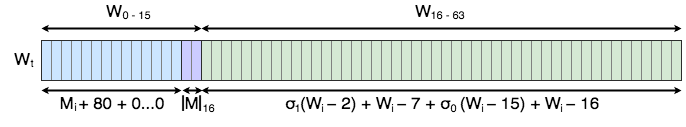
\includegraphics[scale=0.5]{img/SHA-256-Wt.png}
            \caption{Representación gráfica de $W_{t}$}
        \end{figure}

    \subsection{Los primeros 16 registros de $W_t$}
        En el primer intervalo de $W_{t}$ se reservan los 16 primeros registros para almacenar el mensaje de entrada $M$ en formato hexadecimal dividido en bloques de 32 bits. Tiene un tamaño o longitud de 512 bits. En el punto 2 de este documento se explica que el mensaje de entrada $M$ puede tener una longitud variable, e incluso no tener longitud (cadena vacía). Sea cual sea la longitud, se ha de utilizar su representación hexadecimal, y se ha de dividir en palabras de 32 bits de izquierda a derecha. Si alguno de los bloques no llega a ocupar los 32 bits, los bits restantes se han de dejar vacíos para completarlos más adelante.
            \begin{figure}[H]
            \centering
                $Hola \ mundo = \overbrace{\texttt{486f6c61}}^{32 \ bits} \ \overbrace{\texttt{206d756e}}^{32 \ bits} \ \overbrace{\texttt{646f\ \ \ \ }}^{32 \ bits}$
            \end{figure}
        
        A continuación hay que tomar un bit que represente el número 1 decimal o base 10, es decir $00000001$, este se desplaza al bit más alto del byte, con lo que se obtiene $10000000$ y finalmente se calcula el valor hexadecimal, que es $80$.
            \begin{figure}[H]
            \centering
                $10000000_{2} = \texttt{80}_{16}$
            \end{figure}
        
        Independientemente de la longitud de cadena hexadecimal de la palabra de entrada, se añade $80$ por la derecha.
            \begin{figure}[H]
            \centering
                $\texttt{486f6c61} + \texttt{206d756e} + \texttt{646f} + \texttt{80}$
            \end{figure}
        
        Ahora hay que añadir a la cadena una cantidad de bits con valor $0$ hasta llegar a 448 bits en total, que es la longitud que abarca todos los intervalos que van desde $W_{0}$ hasta $W_{13}$.
            \begin{figure}[H]
            \centering
                $\left .
                \begin{array}{l}
                    \overbrace{\texttt{486f6c61}}^{32 \ bits}+\overbrace{\texttt{206d756e}}^{32 \ bits}+\overbrace{\texttt{646f} + \texttt{80} + \texttt{00}}^{32 \ bits}+ \\
                    \texttt{00000000}+\texttt{00000000}+\texttt{00000000}+ \\
                    \texttt{00000000}+\texttt{00000000}+\texttt{00000000}+ \\
                    \texttt{00000000}+\texttt{00000000}+\texttt{00000000}+ \\
                    \texttt{00000000}+\texttt{00000000}
                \end{array}
                \right \} = \texttt{448} \ bits$
            \end{figure}

        Para terminar de completar $W_{t}$ solo queda rellenar los últimos dos bloques de 32 bits $W_{14}$ y $W_{15}$ con la longitud del mensaje de entrada $|M|$ en hexadecimal, con tantos ceros por la izquierda como sean necesario para alcanzar 64 bits de longitud. La obtención de este dato se explica en el punto 2.2 de este documento.
            \begin{figure}[H]
            \centering
                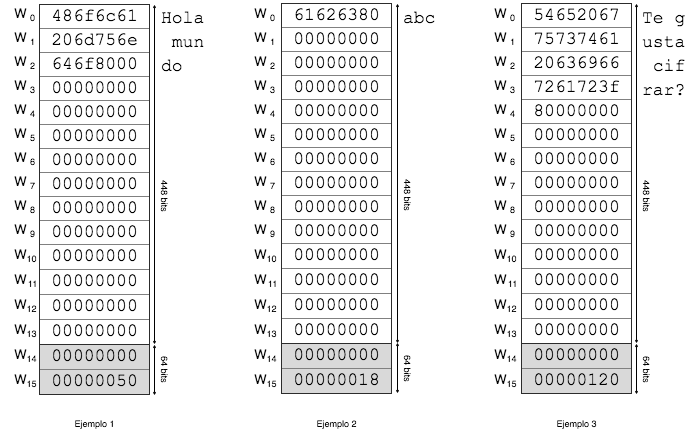
\includegraphics[scale=0.49]{img/SHA-256-W0-W15}
                \caption{Tres ejemplos distintos de esquemas de relleno para las 16 primeras posiciones de $W_{t}$.}
            \end{figure}
    
\section{Constante $K_{t}$}
    La constante $K_{t}$ se compone de $64$ palabras hexadecimales. Cada una de esas palabras representa los 32 primeros bits (en hexadecimal) de la parte fraccionaria de la raíz cúbica de cada uno de los primeros 64 números primos. Estos números primos son:
        \begin{figure}[H]
        \centering
        $\begin{array}{llllllllllllllll}
            2 & 3 & 5 & 7 & 11 & 13 & 17 & 19 & 23 & 29 & 31 & 37 & 41 \\
            43 & 47 & 53 & 59 & 61 & 67 & 71 & 73 & 79 & 83 & 89 & 97 & 101 \\
            103 & 107 & 109 & 113 & 127 & 131 & 137 & 139 & 149 & 151 & 157 & 163 & 167 \\
            173 & 179 & 181 & 191 & 193 & 197 & 199 & 211 & 223 & 227 & 229 & 233 & 239 \\
            241 & 251 & 257 & 263 & 269 & 271 & 277 & 281 & 283 & 293 & 307 & 311 & 
        \end{array}$
        \end{figure}
    
    Se puede representar en código C la constante de tipo array de 64 elementos con su valor inicial de la siguiente forma:
        \begin{figure}[H]
        \centering
            \begin{minted}{c}
    static const unsigned int k[64] = {
    	0x428a2f98, 0x71374491, 0xb5c0fbcf, 0xe9b5dba5,
    	0x3956c25b, 0x59f111f1, 0x923f82a4, 0xab1c5ed5,
    	0xd807aa98, 0x12835b01, 0x243185be, 0x550c7dc3,
    	0x72be5d74, 0x80deb1fe, 0x9bdc06a7, 0xc19bf174,
    	0xe49b69c1, 0xefbe4786, 0x0fc19dc6, 0x240ca1cc,
    	0x2de92c6f, 0x4a7484aa, 0x5cb0a9dc, 0x76f988da,
    	0x983e5152, 0xa831c66d, 0xb00327c8, 0xbf597fc7,
    	0xc6e00bf3, 0xd5a79147, 0x06ca6351, 0x14292967,
    	0x27b70a85, 0x2e1b2138, 0x4d2c6dfc, 0x53380d13,
    	0x650a7354, 0x766a0abb, 0x81c2c92e, 0x92722c85,
    	0xa2bfe8a1, 0xa81a664b, 0xc24b8b70, 0xc76c51a3,
    	0xd192e819, 0xd6990624, 0xf40e3585, 0x106aa070,
    	0x19a4c116, 0x1e376c08, 0x2748774c, 0x34b0bcb5,
    	0x391c0cb3, 0x4ed8aa4a, 0x5b9cca4f, 0x682e6ff3,
    	0x748f82ee, 0x78a5636f, 0x84c87814, 0x8cc70208,
    	0x90befffa, 0xa4506ceb, 0xbef9a3f7, 0xc67178f2
    };
            \end{minted}
        \end{figure}

    \subsection{Cálculo de las 64 palabras de $K_{t}$}
        Para obtener cada una de las palabras hexadecimales se han de seguir las siguientes operaciones:
        \begin{enumerate}
            \item En primer lugar se toma el primer número primo de lista de 64 números primos, el número $2$, y se obtiene la parte fraccionaria de la raíz cúbica del mismo.
                \begin{figure}[H]
                \centering
                    $\lfloor \sqrt[3]{2} \rfloor = 0.259921049894873$
                \end{figure}
                Una vez se obtiene el resultado se reserva a parte para utilizarlo más adelante.
            
            \item Por otro lado se toma del vector $K$ la primera palabra $K_{0}$, es decir $0x428a2f98$, y se convierte a decimal o base 10.
                \begin{figure}[H]
                \centering
                    $\texttt{0x428a2f98} = \frac{4}{16^{1}} + \frac{2}{16^{2}} + \frac{8}{16^{3}} + \frac{10(a)}{16^{4}} + \frac{2}{16^{5}} + \frac{15(f)}{16^{6}} + \frac{9}{16^{7}} + \frac{8}{16^{8}}$
                \end{figure}
                \begin{figure}[H]
                \centering
                    $\left .
                    \begin{array}{llllr}
                    \vspace{2mm}
                    \frac{4}{16^{1}} & = \frac{4}{16} & = & 0.25 \\ \vspace{2mm}
                    \frac{2}{16^{2}} & = \frac{2}{256} & = & 0.0078125 \\ \vspace{2mm}
                    \frac{8}{16^{3}} & = \frac{8}{4096} & = & 0.001953125 \\ \vspace{2mm}
                    \frac{10}{16^{4}} & = \frac{10}{65536} & = & 0.00015258789063 \\ \vspace{2mm}
                    \frac{2}{16^{5}} & = \frac{2}{1048576} & = & 0.00000190734863 \\ \vspace{2mm}
                    \frac{15}{16^{6}} & = \frac{15}{16777216} & = & 0.00000089406967 \\ \vspace{2mm}
                    \frac{9}{16^{7}} & = \frac{9}{268435456} & = & 0.00000003352761 \\ \vspace{2mm}
                    \frac{8}{16^{8}} & = \frac{8}{4294967296} & = & 0.00000000186265
                    \end{array}
                    \right \} \Sigma = 0.25992104969919$
                \end{figure}
            
            \item Se puede observar que los resultados obtenidos en los puntos 1 y 2 de esta sección se aproximan.
                \begin{figure}[H]
                \centering
                    $0.259921049894873 \approx 0.25992104969919$
                \end{figure}
            
            \item Por último hay que representar estos dos números decimales o base 10 en sistema hexadecimal o base 16, y tomar solo los primeros 32 bits, en cuyo caso ambos son iguales.
                \begin{figure}[H]
                \centering
                    $\begin{array}{lcl}
                    0.25992104969919_{10} & = & \texttt{0.}\underbrace{\texttt{428a2f98}}_{32 \ bits}\texttt{0000c4163f52}_{16} \\
                    0.259921049894873_{10} & = & \texttt{0.}\underbrace{\texttt{428a2f98}}_{32 \ bits}\texttt{d728a242d2b4}_{16}
                    \end{array}$
                \end{figure}
            
            \item Por lo tanto se puede decir que $0x428a2f98 = \lfloor \sqrt[3]{2} \rfloor$.
            \vspace{3mm}
        \end{enumerate}
        
        Para comprobar las otras 63 palabras hexadecimales solo hay que repetir los cálculos de los puntos anteriores con cada uno de los 63 números primos restantes, y comprobar su equivalencia respectiva con las palabras de la constante $K_{t}$:
            \begin{figure}[H]
            \centering
                $\begin{array}{lccl}
                    K_{0} & \texttt{0x428a2f98} & = & \lfloor \sqrt[3]{2} \rfloor \\
                        K_{1} & \texttt{0x71374491} & = & \lfloor \sqrt[3]{3} \rfloor \\
                    K_{2} & \texttt{0xb5c0fbcf} & = & \lfloor \sqrt[3]{5} \rfloor \\
                    K_{3} & \texttt{0xe9b5dba5} & = & \lfloor \sqrt[3]{7} \rfloor \\
                    & \vdots & \\
                    K_{63} & \texttt{0xc67178f2} & = & \lfloor \sqrt[3]{311} \rfloor
                \end{array}$
            \end{figure}

\section{Las 8 palabras iniciales}
    La función SHA-256 utiliza una grupo inicial de 8 palabras correlacionadas una a una con las variables $A$, $B$, $C$, $D$, $E$, $F$, $G$ y $H$. Cada una de estas palabras representa los 32 primeros bits en hexadecimal o base 16 de la parte fraccionaria de las raíces cuadradas de los primeros 8 números primos. Se trata de los 8 valores iniciales que se reciben en la primera ronda criptográfica y que se asignarán a un vector de 8 elementos denominado $P_{t}$, donde:
        \begin{figure}[H]
        \centering
            $\begin{array}{llll}
                P_{0} = A & P_{1} = B & P_{2} = C & P_{3} = D \\
                P_{4} = E & P_{5} = F & P_{6} = G & P_{7} = H
            \end{array}$
        \end{figure}
    
    Se puede representar en código C la constante de tipo array de 8 elementos con su valor inicial de la siguiente forma:
        \begin{figure}[H]
        \centering
            \begin{minted}{c}
    unsigned int p[8] = {
    	0x6a09e667, 0xbb67ae85, 0x3c6ef372,
    	0xa54ff53a, 0x510e527f, 0x9b05688c,
    	0x1f83d9ab, 0x5be0cd19
    };
            \end{minted}
        \end{figure}
    
    Los 8 valores iniciales son siempre los mismos únicamente en la primera ronda criptográfica. En las siguientes rondas estas palabras irán cambiando cíclicamente su valor de entrada.
    
    \subsection{Cálculo de las 8 palabras iniciales}
        Para obtener estas 8 palabras de la primera ronda criptográfica se deben seguir las siguientes operaciones:
        \begin{enumerate}
            \item Se toman los 8 primeros números primos, es decir, $2$, $3$, $5$, $7$, $11$, $13$, $17$ y $19$. A continuación se obtiene la raíz cuadrada de cada uno de ellos y se reserva únicamente la parte fraccionaria.
                \begin{figure}[H]
                \centering
                    $\begin{array}{lcl}
                        \sqrt[2]{2} \approx 1.4142135623730950 & \rightarrow & \lfloor \sqrt[2]{2} \rfloor \approx 0.4142135623730950 \\
                        \sqrt[2]{3} \approx 1.7320508075688770 & \rightarrow & \lfloor \sqrt[2]{3} \rfloor \approx 0.7320508075688770 \\
                        \sqrt[2]{5} \approx 2.2360679774997900 & \rightarrow & \lfloor \sqrt[2]{5} \rfloor \approx 0.2360679774997900 \\
                        \sqrt[2]{7} \approx 2.6457513110645910 & \rightarrow & \lfloor \sqrt[2]{7} \rfloor \approx 0.6457513110645910 \\
                        \sqrt[2]{11} \approx 3.316624790355400 & \rightarrow & \lfloor \sqrt[2]{11} \rfloor \approx 0.316624790355400 \\
                        \sqrt[2]{13} \approx 3.605551275463989 & \rightarrow & \lfloor \sqrt[2]{13} \rfloor \approx 0.605551275463989 \\
                        \sqrt[2]{17} \approx 4.123105625617661 & \rightarrow & \lfloor \sqrt[2]{17} \rfloor \approx 0.123105625617661 \\
                        \sqrt[2]{19} \approx 4.358898943540674 & \rightarrow & \lfloor \sqrt[2]{19} \rfloor \approx 0.358898943540674
                    \end{array}$
                \end{figure}
            
            \item Se convierte la parte fraccionaria de sistema decimal o base 10 a hexadecimal o base 16.
                \begin{figure}[H]
                \centering
                    $\begin{array}{lcl}
                        0.414213562373095_{10} & = & \texttt{0.6A09E667}_{16} \\
                        0.732050807568877_{10} & = & \texttt{0.BB67AE85}_{16} \\
                        0.236067977499790_{10} & = & \texttt{0.3C6EF372}_{16} \\
                        0.645751311064591_{10} & = & \texttt{0.A54FF53A}_{16} \\
                        0.316624790355400_{10} & = & \texttt{0.510E527F}_{16} \\
                        0.605551275463989_{10} & = & \texttt{0.9B05688C}_{16} \\
                        0.123105625617661_{10} & = & \texttt{0.1F83D9AB}_{16} \\
                        0.358898943540674_{10} & = & \texttt{0.5BE0CD19}_{16}
                    \end{array}$
                \end{figure}
            
            \item Finalmente se almacena únicamente la parte fraccionaria hexadecimal como las 8 palabras de entrada A, B, C, D, E, F, G y H.
                \begin{figure}[H]
                \centering
                    $\begin{array}{rclcrcl}
                        A & = & \texttt{0x6A09E667} & \ & E & = & \texttt{0x510E527F} \\
                        B & = & \texttt{0xBB67AE85} & \ & F & = & \texttt{0x9B05688C} \\
                        C & = & \texttt{0x3C6EF372} & \ & G & = & \texttt{0x1F83D9AB} \\
                        D & = & \texttt{0xA54FF53A} & \ & H & = & \texttt{0x5BE0CD19}
                    \end{array}$
                \end{figure}
        \end{enumerate}

\section{Primera ronda criptográfica}
    Habiendo calculado anteriormente las 8 palabras iniciales $A$, $B$, $C$, $D$, $E$, $F$, $G$ y $H$, las 64 palabras variables de $W_{t}$ y conociendo las 64 palabras constantes de $K_{t}$, ya se tienen los elementos necesarios para realizar la primera ronda criptográfica. Para ello es necesario seguir estrictamente unas reglas y funciones que se detallan en los siguientes puntos. El siguiente diagrama muestra los movimientos y funciones por los que ha de pasar cada una de las 8 palabras iniciales en cada ronda, hasta completar 64 rondas.
        \begin{figure}[H]
        \centering
            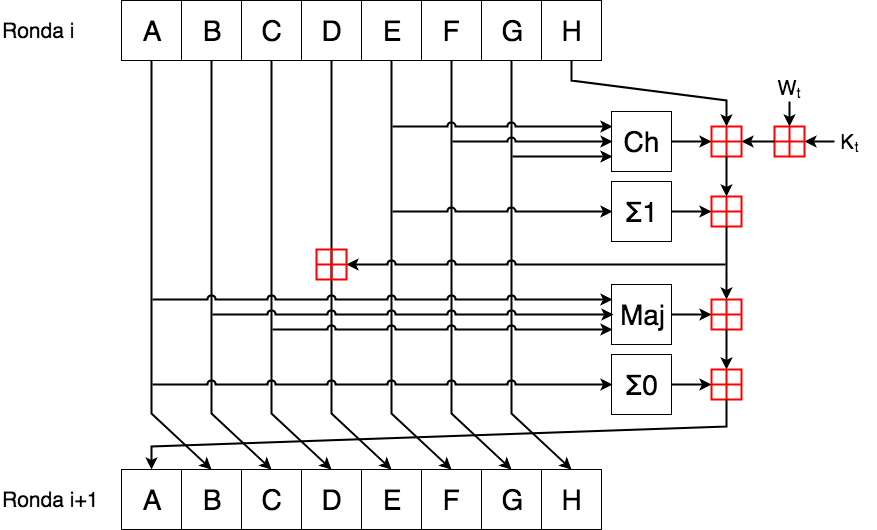
\includegraphics[scale=0.33]{img/SHA-256-diagram.png}
            \caption{Diagrama del funcionamiento cíclico de SHA-256}
        \end{figure}
    
    Los recuadros de color rojo del diagrama representan una suma $mod \ 2^{32}$, o lo que es lo mismo, una suma binaria de los inputs de 32 bits que reciba sin tener en cuanta las unidades que se deban llevar al siguiente nivel.
    
    \subsection{Operaciones con las 8 palabras}
        En la primera ronda criptográfica las palabras $A$, $B$, $C$, $D$, $E$, $F$, $G$ y $H$ tendrán siempre el mismo valor inicial, tal y como se explica en el punto 5 de este documento. Hay que hacer una serie de operaciones y movimientos con los valores de cada una de las palabras, de modo que se obtenga un nuevo valor de las mismas para la siguiente ronda. Es decir, en la primera ronda $A_{0}$ siempre tendrá como valor $6A09E667$, pero en la segunda ronda $A_{1}$ tendrá un valor muy distinto, dependerá del resultado de una serie de movimientos y operaciones, y esto sucederá con el todas y cada una de las palabras.
        
        \subsubsection{Operaciones con $A$}
            La palabra $A$ se va a utilizar en tres casos por cada ronda:
            \begin{itemize}
                \item El valor actual de $A_{i}$ será el nuevo valor que tendrá la palabra $B_{i+1}$ en la siguiente ronda. En este caso no se hace ningún cálculo, solo se transfiere el valor.
                \begin{figure}[H]
                \centering
                    $A_{i} \Rightarrow B_{i+1}$
                \end{figure}
                \item Se pasa como argumento a la función $Maj$ y se utilizará para obtener el nuevo valor de $A_{i+1}$ en la siguiente ronda.
                \item Se pasa como argumento a la función $\Sigma0$ y también se utilizará como elemento para calcular el nuevo valor de $A_{i+1}$ en la siguiente ronda.
            \end{itemize}
        
        \subsubsection{Operaciones con $B$ y $C$}
            Las palabras $B$ y $C$ se van a utilizar cada una en dos casos por cada ronda:
            \begin{itemize}
                \item El valor actual de $B_{i}$ será el nuevo valor que tendrá la palabra $C_{i+1}$, y el valor de $C_{i}$ será el nuevo valor que tendrá $D_{i+1}$ en la siguiente ronda. En este caso no se hace ningún cálculo, solo se transfiere el valor.
                \begin{figure}[H]
                \centering
                    $B_{i} \Rightarrow C_{i+1} \qquad C_{i} \Rightarrow D_{i+1}$
                \end{figure}
                \item Sendos valores $B_{i}$ y $C_{i}$ se pasan como argumento a la función $Maj$ para obtener el nuevo valor de $A_{i+1}$ en la siguiente ronda.
            \end{itemize}
        
        \subsubsection{Operaciones con $D$}
            La palabra $D$ se va a utilizar en un único caso por cada ronda. Su valor actual $D_{i}$ será un elemento más en la operación $mod \ 2^{32}$ junto con los valores de $W_{t}$, $K_{t}$, $H_{i}$, el resultado de la función $Ch$ y el resultado de la función $\Sigma1$ para obtener el valor de $E_{i+1}$.
                \begin{figure}[H]
                \centering
                    $mod \ 2^{32} (W_{t}, K_{t}, H_{i}, Ch, \Sigma1, D_{i}) = E_{i+1}$
                    
                    \begin{figure}[H]
                    \centering
                        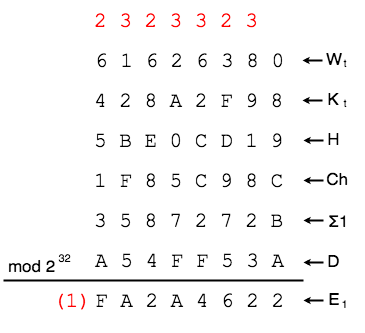
\includegraphics[scale=0.41]{img/SHA-256-operations_D.png}
                        \caption{La operación $mod \ 2^{32}$ con $W_{t}$, $K_{t}$, $H$, $Ch$, $\Sigma1$ y $D$.}
                    \end{figure}
                \end{figure}
            El ejemplo anterior muestra los datos con los que se ha de operar en la primera ronda criptográfica para el mensaje de entrada $M = "abc"$. El resultado que se obtiene es el valor que tendrá $E_{1}$ (la palabra $E$ en la segunda ronda). Los números en color rojo de la parte superior son el acarreo de la suma de cada carácter hexadecimal, y el número rojo de la parte inferior izquierda es el número hexadecimal que es excluido.
            
        \subsubsection{Operaciones con $E$}
            La palabra $E$ se va a utilizar en tres casos por cada ronda:
            \begin{itemize}
                \item El valor actual de $E_{i}$ será el nuevo valor que tendrá la palabra $F_{i+1}$ en la siguiente ronda. En este caso no se hace ningún cálculo, solo se transfiere el valor.
                \begin{figure}[H]
                \centering
                    $E_{i} \Rightarrow F_{i+1}$
                \end{figure}
                \item Se pasa como argumento a la función $Ch$ para obtener el nuevo valor de $A_{i+1}$ en la siguiente ronda.
                \item Se pasa como argumento a la función $\Sigma1$ y también se utilizará como elemento para calcular el nuevo valor de $A_{i+1}$ en la siguiente ronda.
            \end{itemize}
        
        \subsubsection{Operaciones con $F$ y $G$}
            Las palabras $F$ y $G$ se van a utilizar cada una en dos casos por cada ronda:
            \begin{itemize}
                \item El valor actual de $F_{i}$ será el nuevo valor que tendrá la palabra $G_{i+1}$, y el valor de $G_{i}$ será el nuevo valor que tendrá $H_{i+1}$ en la siguiente ronda. En este caso no se hace ningún cálculo, solo se transfiere el valor.
                \begin{figure}[H]
                \centering
                    $F_{i} \Rightarrow G_{i+1} \qquad G_{i} \Rightarrow H_{i+1}$
                \end{figure}
                \item Sendos valores $F_{i}$ y $G_{i}$ se pasan como argumento a la función $Ch$ para obtener el nuevo valor de $A_{i+1}$ en la siguiente ronda.
            \end{itemize}
        
        \subsubsection{Operaciones con $H$}
            La palabra $H$ se va a utilizar en un único caso por cada ronda. Su valor actual será un elemento más en la operación $mod \ 2^{32}$ junto con los valores de $W_{t}$, $K_{t}$, el resultado de las funciones $Ch$, $\Sigma1$, $Maj$ y $\Sigma0$ para obtener el valor de $A_{i+1}$
        
    \subsection{Función $Ch$}
        Se trata de una función booleana que realizará operaciones lógicas tomando como datos de entrada las palabras $E$, $F$ y $G$. Se opera con cada bit de la palabra hexadecimal aplicando la siguiente fórmula de lógica proposicional:
            \begin{figure}[H]
            \centering
                $Ch(E, F, G) = (E \land F) \lor (\lnot E \land G)$
            \end{figure}
            \begin{table}[H]
            \centering
            \begin{tabular}{| c c c | c c c |} 
                \hline
                $E$ & $F$ & $G$ & $(E \land F)$ & $\lor$ & $(\lnot E \land G)$ \\
                \hline
                1 & 1 & 1 & 1 & \textbf1 & 0 \\
                1 & 1 & 0 & 1 & \textbf1 & 0 \\
                1 & 0 & 1 & 0 & \textbf0 & 0 \\
                1 & 0 & 0 & 0 & \textbf0 & 0 \\
                0 & 1 & 1 & 0 & \textbf1 & 1 \\
                0 & 1 & 0 & 0 & \textbf0 & 0 \\
                0 & 0 & 1 & 0 & \textbf1 & 1 \\
                0 & 0 & 0 & 0 & \textbf0 & 0 \\
                \hline
            \end{tabular}
            \caption{\textit{Tabla de la verdad de la función $Ch$}}
            \label{table:1}
            \end{table}
        En el \textit{álgebra de Boole}\footnote{Álgebra de Boole: https://en.wikipedia.org/wiki/Boolean\_algebra} la anterior tabla se denomina \textit{tabla de la verdad}, y en este caso representa las 16 posibilidades binarias existentes en el caso de un input de tres entradas $\delta_{x}$, $\delta_{y}$ y $\delta_{z}$. Además muestra el resultado en cada una de las posibilidades para la operación lógica $(\delta_{x} \land \delta_{y}) \lor (\lnot \delta_{x} \land \delta_{z})$.
        
        \vspace{3mm}
        En la primera ronda criptográfica los valores de las palabras $E$, $F$ y $G$ son constantes, tal y como se indica en el punto 5.1 de este documento. El resultado de la función $Ch(E_{0}, F_{0}, G_{0})$ es el siguiente:
            \begin{figure}[H]
            \centering
                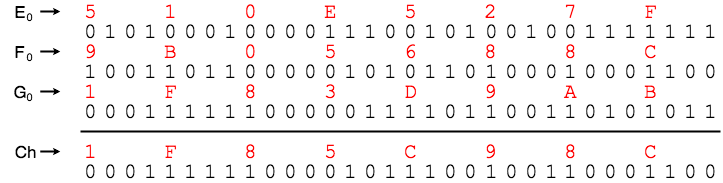
\includegraphics[scale=0.41]{img/SHA-256-function_Ch.png}
                \caption{Cálculo bit a bit para $(E_{0} \land F_{0}) \lor (\lnot E_{0} \land G_{0})$}
            \end{figure}
        Se puede comprobar en la \textit{tabla de la verdad} los resultados de las operaciones de 3 bits en cada caso. El resultado siempre se expresará en hexadecimal.
            \begin{figure}[H]
            \centering
                $Ch_{0} = \texttt{0x1F85C98C}$
            \end{figure}
        
    \subsection{Función $\Sigma1$}
        Esta función realiza una serie de operaciones binarias rotativas $ROT$ y operaciones lógicas $XOR$ teniendo como input el valor de $E_{i}$ en cada ronda criptográfica. La fórmula para cada bit $x$ es la siguiente:
            \begin{figure}[H]
            \centering
                $\Sigma1(x) = ROT \ R^{6}(x) \oplus ROT \ R^{11}(x) \oplus ROT \ R^{25}(x)$
            \end{figure}
        Tal y como se explica en el punto 5.1 de este documento, la palabra $E_{0}$ es una constante con valor hexadecimal $0x510E527F$ únicamente en la primera ronda. A continuación un ejemplo del cálculo de la función $\Sigma1_{0}$.
            \begin{figure}[H]
            \centering
                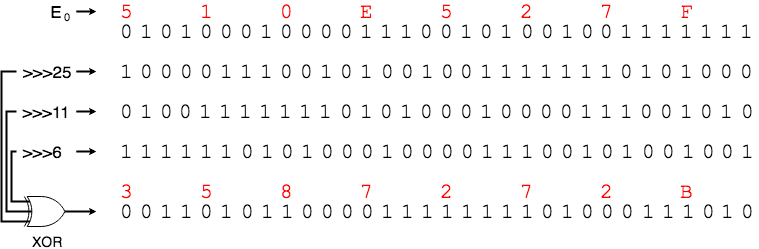
\includegraphics[scale=0.41]{img/SHA-256-function_Sigma1.png}
                \caption{Cálculo bit a bit para $ROT \ R^{6}(x) \oplus ROT \ R^{11}(x) \oplus ROT \ R^{25}(x)$}
            \end{figure}
        En el ejemplo anterior se realiza una operación $XOR$ de tres inputs, que son cada uno de los bits de $E_{0}$ tras realizar una operación de rotación de 25 bits a la derecha, 11 bits a la derecha y 6 bits a la derecha también. El resultado siempre se expresará en hexadecimal.
            \begin{figure}[H]
            \centering
                $\Sigma1_{0} = \texttt{0x3587272B}$
            \end{figure}
        
    \subsection{Función $Maj$}
        Se trata de una función booleana que realizará operaciones lógicas tomando como datos de entrada las palabras $A$, $B$ y $C$. Se opera con cada bit de la palabra hexadecimal aplicando la siguiente fórmula de lógica proposicional:
            \begin{figure}[H]
            \centering
                $Maj(A, B, C) = (A \land B) \lor (A \land C) \lor ( B \land C)$
            \end{figure}
            \begin{table}[H]
            \centering
            \begin{tabular}{| c c c | c c c c c |} 
                \hline
                $A$ & $B$ & $C$ & $(A \land B)$ & $\lor$ & $(A \land C)$ & $\lor$ & $( B \land C)$ \\
                \hline
                1 & 1 & 1 & 1 & 1 & 1 & \textbf1 & 1 \\
                1 & 1 & 0 & 1 & 1 & 0 & \textbf1 & 0 \\
                1 & 0 & 1 & 0 & 1 & 1 & \textbf1 & 0 \\
                1 & 0 & 0 & 0 & 0 & 0 & \textbf0 & 0 \\
                0 & 1 & 1 & 0 & 0 & 0 & \textbf1 & 1 \\
                0 & 1 & 0 & 0 & 0 & 0 & \textbf0 & 0 \\
                0 & 0 & 1 & 0 & 0 & 0 & \textbf0 & 0 \\
                0 & 0 & 0 & 0 & 0 & 0 & \textbf0 & 0 \\
                \hline
            \end{tabular}
            \caption{\textit{Tabla de la verdad de la función $Maj$}}
            \label{table:2}
            \end{table}
        La tabla anterior muestra el resultado en cada una de las 16 posibilidades binarias para la operación lógica $(\delta_{x} \land \delta_{y}) \lor (\delta_{x} \land \delta_{z}) \lor (\delta_{y} \land \delta_{z})$.
        
        \vspace{3mm}
        En la primera ronda criptográfica los valores de las palabras $A$, $B$ y $C$ son constantes, tal y como se indica en el punto 5.1 de este documento. El resultado de la función $Maj(A_{0}, B_{0}, C_{0})$ es el siguiente:
            \begin{figure}[H]
            \centering
                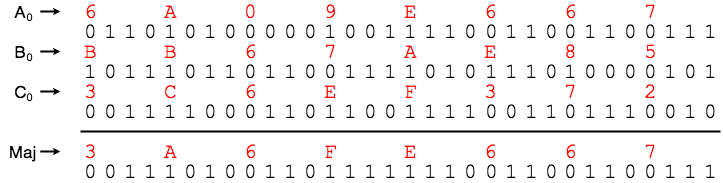
\includegraphics[scale=0.41]{img/SHA-256-function_Maj.png}
                \caption{Cálculo bit a bit para $(A_{0} \land B_{0}) \lor (A_{0} \land C_{0}) \lor (B_{0} \land C_{0})$}
            \end{figure}
        El resultado siempre se expresará en hexadecimal.
            \begin{figure}[H]
            \centering
                $Maj_{0} = \texttt{0x3A6FE667}$
            \end{figure}
        
    \subsection{Función $\Sigma0$}
        Al igual que la función $\Sigma1$ esta función realiza una serie de operaciones binarias rotativas $ROT$ y operaciones lógicas $XOR$ teniendo como input el valor de $A_{i}$ en cada ronda criptográfica. La fórmula para cada bit $x$ es la siguiente:
            \begin{figure}[H]
            \centering
                $\Sigma0(x) = ROT \ R^{2}(x) \oplus ROT \ R^{13}(x) \oplus ROT \ R^{22}(x)$
            \end{figure}
        Tal y como se explica en el punto 5.1 de este documento, la palabra $A_{0}$ es una constante con valor hexadecimal $0x6A09E667$ únicamente en la primera ronda. A continuación un ejemplo del cálculo de la función $\Sigma0_{0}$.
            \begin{figure}[H]
            \centering
                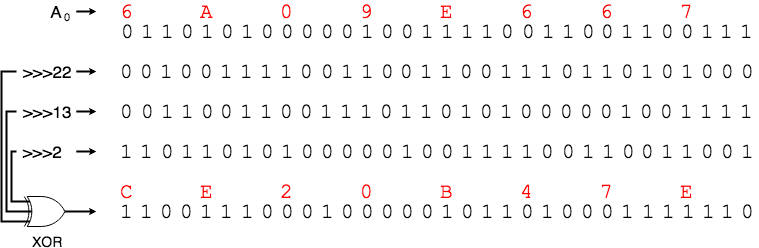
\includegraphics[scale=0.41]{img/SHA-256-function_Sigma0.png}
                \caption{Cálculo bit a bit para $ROT \ R^{2}(x) \oplus ROT \ R^{13}(x) \oplus ROT \ R^{22}(x)$}
            \end{figure}
        En el ejemplo anterior se realiza una operación $XOR$ de tres inputs, que son cada uno de los bits de $A_{0}$ tras realizar una operación de rotación de 2 bits a la derecha, 13 bits a la derecha y 22 bits a la derecha también. El resultado siempre se expresará en hexadecimal.
            \begin{figure}[H]
            \centering
                $\Sigma1_{0} = \texttt{0xCE20B47E}$
            \end{figure}
    
    \subsection{Las 8 nuevas palabras resultantes}
        Como resultado de las anteriores operaciones se obtienen los nuevos valores de las 8 palabras $A$, $B$, $C$, $D$, $E$, $F$, $G$ y $H$ para las siguiente ronda.
            \begin{figure}[H]
            \centering
                $\begin{array}{lcl}
                    A_{i+1} & = & mod \ 2^{32} (W_{t}, K_{t}, Ch, \Sigma1, Maj, \Sigma0) \\
                    B_{i+1} & = &  A_{i} \\
                    C_{i+1} & = &  B_{i} \\
                    D_{i+1} & = &  C_{i} \\
                    E_{i+1} & = &  mod \ 2^{32} (W_{t}, K_{t}, H_{i}, Ch, \Sigma1, D_{i}) \\
                    F_{i+1} & = &  E_{i} \\
                    G_{i+1} & = &  F_{i} \\
                    H_{i+1} & = &  G_{i} \\
                \end{array}$
            \end{figure}
        
\section{Siguientes rondas}
    En total se han de realizar 64 rondas, y en cada ronda las 8 palabras $A$, $B$, $C$, $D$, $E$, $F$, $G$ y $H$ irán tomando nuevos valores. Una vez terminadas todas las rondas criptográficas, antes de obtener la cadena \textit{digest} del mensaje original $M$ primero se han de sumar los valores de la palabra correspondiente a la primera ronda $P_{0}$ y la última $P_{63}$ en una operación $mod \ 2^{32}$, por ejemplo, para los datos de entrada $M = "abc"$:
        \begin{figure}[H]
        \centering
            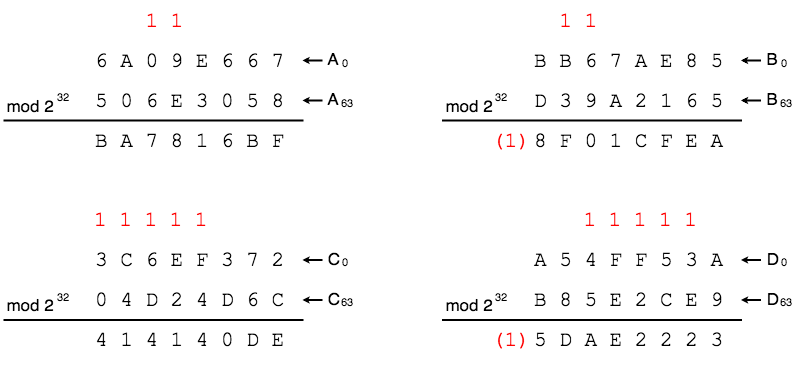
\includegraphics[scale=0.41]{img/SHA-256-last_calculation_0.png}
        \end{figure}
        \begin{figure}[H]
        \centering
            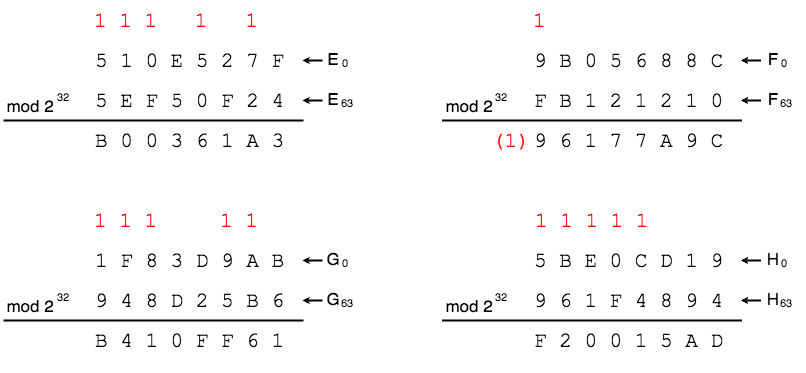
\includegraphics[scale=0.41]{img/SHA-256-last_calculation_1.png}
            \caption{Cálculo bit a bit $mod \ 2^{32}$ de las palabras $P_{0}$ y $P_{63}$.}
        \end{figure}
    Finalmente se han de concatenar los resultados de las operaciones anteriores de la siguiente manera:
        \begin{figure}[H]
        \centering
            $A+B+C+D+E+F+G+H = \left \{
                \begin{array}{c}
                    \texttt{ba7816bf8f01cfea414140de5dae2223} \\
                    \texttt{b00361a396177a9cb410ff61f20015ad}
                \end{array}
                \right .$
        \end{figure}
    Así pues, el \textit{hash} o \textit{digest} resultante para la cadena o datos de entrada "\textit{abc}" será siempre la misma cadena de 256 bits de longitud expresada en 64 caracteres hexadecimales o base 16.
        \begin{figure}[H]
        \centering
            $sha256('abc') = \left \{
                \begin{array}{c}
                    \texttt{ba7816bf8f01cfea414140de5dae2223} \\
                    \texttt{b00361a396177a9cb410ff61f20015ad}
                \end{array}
                \right .$
        \end{figure}
\end{document}

